\documentclass[12pt,a4paper,openany]{book}

\usepackage[a4paper,left=1.25in,right=1in,top=1in,bottom=1in]{geometry}
\usepackage{iftex}
\ifLuaTeX
  \usepackage{fontspec}
  \defaultfontfeatures{Ligatures=TeX,Renderer=HarfBuzz}
  \setmainfont{Latin Modern Roman}
  \newfontfamily\banglafont[Script=Bengali,Language=Bengali]{Noto Serif Bengali}
  \newcommand{\bn}[1]{{\banglafont #1}}
\else
  \usepackage[utf8]{inputenc}
  \newcommand{\bn}[1]{#1}
\fi
\usepackage{setspace}
\usepackage{graphicx}
\usepackage{booktabs}
\usepackage{longtable}
\usepackage{array}
\usepackage{multirow}
\usepackage{amsmath}
\usepackage{amssymb}
\usepackage{float}
\usepackage{placeins}
\usepackage{enumitem}
\usepackage{xcolor}
\usepackage{caption}
\usepackage{subcaption}
\usepackage{listings}
\usepackage{tikz}
\usetikzlibrary{arrows.meta,positioning,shapes.geometric,shapes.misc,fit,calc}
\usepackage[hidelinks]{hyperref}
\usepackage{cite}

\setstretch{1.35}
\setlength{\parindent}{0.35in}
\setlength{\parskip}{0.25em}
\emergencystretch=2em

\captionsetup{font=small,labelfont=bf}
\renewcommand{\arraystretch}{1.18}

\lstdefinestyle{codeblock}{
  basicstyle=\ttfamily\small,
  breaklines=true,
  frame=single,
  columns=fullflexible,
  keepspaces=true,
  showstringspaces=false,
  tabsize=2
}
\lstset{style=codeblock}

\newcommand{\thesistitle}{AI-Enhanced Complaint Management System for Government Marketplaces}
\newcommand{\studentone}{Syed Mafijul Islam}
\newcommand{\studenttwo}{Nahidur Zaman}
\newcommand{\studentthree}{Sakif Shahrear}
\newcommand{\supervisor}{M. Aktaruzzaman}
\newcommand{\department}{Department of Computer Science \& Engineering}
\newcommand{\institution}{Military Institute of Science and Technology}
\newcommand{\supervisordesignation}{Associate Professor and Head}
\newcommand{\supervisordepartment}{Department of Robotics and Mechatronics Engineering}
\newcommand{\supervisorinstitution}{Daffodil International University}
\newcommand{\submissiondate}{May 2026}

\newcommand{\placeholderbox}[2]{
\begin{figure}[H]
  \centering
  \fbox{\begin{minipage}[c][0.22\textheight][c]{0.86\textwidth}
    \centering
    \textbf{#1}\\[0.75em]
    \small #2
  \end{minipage}}
  \caption{#1}
\end{figure}
}

\begin{document}

\frontmatter

\begin{titlepage}
\begin{center}
{\Large \textbf{\institution}}\\[0.3cm]
{\large \department}\\[2.2cm]

{\Large \textbf{Undergraduate Thesis}}\\[0.6cm]
{\LARGE \textbf{\thesistitle}}\\[2.2cm]

\textbf{Submitted by}\\[0.3cm]
\studentone\\
\studenttwo\\
\studentthree\\[1.4cm]

\textbf{Supervised by}\\[0.3cm]
\supervisor\\
\supervisordesignation\\
\supervisordepartment\\
\supervisorinstitution\\[1.4cm]

\textbf{Submitted in partial fulfillment of the requirements for the degree of}\\[0.2cm]
\textbf{Bachelor of Science in Computer Science and Engineering}\\[1.3cm]

\submissiondate
\end{center}
\end{titlepage}

\chapter*{Declaration}
\addcontentsline{toc}{chapter}{Declaration}
We hereby declare that this thesis titled \textit{\thesistitle} has been completed as part of the undergraduate research requirement. The work presented in this thesis is based on our own design, implementation, experimentation, and analysis, except where external sources have been cited using standard academic conventions.

We further declare that the dataset, experimental results, and machine learning performance values reported in this thesis are not manually invented. The reported evaluation values are obtained from the implemented training pipeline using the 500-complaint dataset exported from the NityMulya backend. Any limitation related to dataset size, backend-feature dependence, class imbalance, or model generalization has been discussed honestly in the relevant chapters.

\vspace{2cm}
\noindent\begin{tabular}{p{0.45\textwidth}p{0.45\textwidth}}
\hrulefill & \hrulefill\\
\studentone & Date\\[1.4cm]
\hrulefill & \hrulefill\\
\studenttwo & Date\\[1.4cm]
\hrulefill & \hrulefill\\
\studentthree & Date
\end{tabular}

\chapter*{Approval Sheet}
\addcontentsline{toc}{chapter}{Approval Sheet}
This thesis titled \textit{\thesistitle}, submitted by \studentone, \studenttwo, and \studentthree, has been accepted as satisfactory in partial fulfillment of the requirements for the degree of Bachelor of Science in Computer Science and Engineering.

\vspace{2.2cm}
\noindent\begin{tabular}{p{0.6\textwidth}p{0.3\textwidth}}
\hrulefill & \hrulefill\\
\supervisor & Date\\
Supervisor\\
\supervisordesignation\\
\supervisordepartment\\
\supervisorinstitution
\end{tabular}

\vspace{2.2cm}
\noindent\begin{tabular}{p{0.6\textwidth}p{0.3\textwidth}}
\hrulefill & \hrulefill\\
Head of Department & Date\\
\department\\
\institution
\end{tabular}

\chapter*{Acknowledgement}
\addcontentsline{toc}{chapter}{Acknowledgement}
We express our sincere gratitude to Almighty Allah for giving us the strength, patience, and opportunity to complete this undergraduate thesis. We are deeply thankful to our supervisor, \supervisor, for his guidance, encouragement, and academic direction throughout the research work.

We also acknowledge the support of our department, teachers, and classmates. Their comments helped us refine the research problem and improve the presentation of the work. Discussions on software engineering, database design, Bengali language processing, and responsible machine learning shaped many parts of this study.

Finally, we thank the people and practical setting behind the NityMulya marketplace platform. Their context gave this work its direction. Our aim was simple: to design a lightweight complaint classification pipeline that can support government marketplace administrators without expensive infrastructure or very large language models.

\chapter*{Abstract}
\addcontentsline{toc}{chapter}{Abstract}
Government marketplaces now depend heavily on digital platforms to receive citizen feedback, monitor service quality, and identify problems in the sale of essential commodities. In Bangladesh, these complaints are often written in Bengali, English, and Banglish. The writing is usually informal. Many complaints are short, mixed-script, and full of spelling variation. Manual review is slow and can become inconsistent when the number of complaints grows. Many public-service systems also work with limited computing resources, so large transformer models may be costly to train, deploy, and maintain.

This work develops a lightweight hybrid Natural Language Processing (NLP) and backend-feature based complaint classification system for the NityMulya government marketplace platform. We used a dataset of 500 complaints stored in a Supabase PostgreSQL backend. Each complaint record contains complaint text, product category, backend validity score, backend priority score, and a severity label from three classes: weak, medium, and high. The pipeline applies Unicode normalization, English and Banglish lowercasing, punctuation cleanup, repeated character normalization, a Banglish normalization dictionary, optional Bengali stopword removal, word-level TF-IDF, character-level TF-IDF, One-Hot Encoding for product category, and scaling for numeric backend features. We compared Logistic Regression, Linear Support Vector Classification, Random Forest, and a Voting ensemble with stratified five-fold cross-validation. We also tested class weighting and SMOTE, while preventing leakage by applying oversampling only inside training folds.

The final selected model is a tuned Logistic Regression classifier that uses normalized complaint text and backend numeric features. On the 20\% stratified test split, it achieved 86.00\% hold-out accuracy and a weighted F1 score of 0.8594. The ablation study gave a clear result: text-only features reached only 0.5559 weighted F1, while text combined with backend validity and priority features reached 0.8503 weighted F1 in cross-validation. Product category features did not help in this dataset and reduced weighted F1. The strongest signal came from feature fusion, especially the combination of text representation with backend decision-support features, not from complaint text alone.

The main contribution is not a large-scale Bengali language model. It is a practical, reproducible, CPU-friendly hybrid pipeline for low-resource government marketplace complaint triage. The study also discusses key concerns: the small dataset, the fact that backend features partly encode operational severity labels, and the limits of generalizing beyond the NityMulya context.

\textbf{Keywords:} Bengali NLP, Banglish normalization, complaint classification, e-governance, TF-IDF, Logistic Regression, Supabase, backend features, lightweight machine learning.

\tableofcontents
\listoffigures
\listoftables

\chapter*{Abbreviation List}
\addcontentsline{toc}{chapter}{Abbreviation List}
\begin{longtable}{p{0.2\textwidth}p{0.7\textwidth}}
\toprule
\textbf{Abbreviation} & \textbf{Meaning}\\
\midrule
API & Application Programming Interface\\
CV & Cross-Validation\\
DBMS & Database Management System\\
F1 & Harmonic mean of precision and recall\\
FN & False Negative\\
FP & False Positive\\
ICT & Information and Communication Technology\\
ML & Machine Learning\\
NFKC & Normalization Form Compatibility Composition\\
NLP & Natural Language Processing\\
OHE & One-Hot Encoding\\
RDBMS & Relational Database Management System\\
RF & Random Forest\\
SMOTE & Synthetic Minority Oversampling Technique\\
SQL & Structured Query Language\\
SVC & Support Vector Classification\\
TF-IDF & Term Frequency-Inverse Document Frequency\\
TN & True Negative\\
TP & True Positive\\
UI & User Interface\\
\bottomrule
\end{longtable}

\mainmatter

\chapter{Introduction}

\section{Background of E-Governance Systems}
E-governance means using information and communication technologies to improve public services. Governments now use digital platforms for citizen registration, subsidy management, online payment, licensing, grievance redress, and marketplace monitoring. Citizens do more than read information on these platforms. They submit feedback, complaints, documents, and evidence. Over time, the platform becomes a steady source of operational data.

Complaint management is a central part of e-governance because it links citizens with administrative action. A complaint may report overpricing, damaged goods, expired products, misleading information, rude shop behavior, or consumer rights violations. Fast handling can build public trust and help administrators find repeated problems. Slow or inconsistent handling has the opposite effect. Citizens may start to see the platform as a form-submission tool, not as a responsive public service.

The NityMulya government marketplace platform is a suitable setting for this research. It supports marketplace information, price awareness, and complaint submission for essential products. Citizens write in everyday language, not in a fixed administrative format. That gives us useful real-world data, but it also creates a technical challenge. The complaint text is often short, informal, mixed-language, and noisy.

\section{Government Marketplace Complaint Management}
Government marketplace complaint management is different from ordinary customer-service ticketing. A commercial help desk usually handles issues between a company and its customers. A government marketplace complaint may involve citizens, shop owners, product categories, legal price ranges, public-health concerns, and administrative enforcement. A complaint about expired milk, false weight, or price manipulation is not only a service issue. It may require regulatory attention.

The usual workflow includes complaint submission, initial review, severity assessment, routing to the responsible authority, investigation, response, and archival. In a manual workflow, administrators read each complaint and decide whether it is weak, medium, or high priority. The decision may depend on the written complaint, the product category, the price context, and backend checks such as whether the charged price exceeded an allowed range. A practical classifier should use that wider context instead of relying on text alone.

\section{Problems in Manual Complaint Processing}
Manual complaint processing creates several operational problems. It is slow. If administrators must read every complaint one by one, the review queue grows as complaint volume increases. Manual classification can also be inconsistent. Different officials may read similar complaints in different ways, especially when the text is informal or incomplete. Pattern detection becomes difficult too. A digital system can count complaints about expired products or overpricing, but those summaries depend on reliable classification.

Another problem is cognitive fatigue. Repeated reading of short complaint texts can lead to shallow review, especially when many entries are similar. A lightweight classifier cannot replace official judgment, but it can provide a first-level severity signal. Administrators can then focus human attention on high-priority complaints while still retaining oversight.

\section{Bengali and Banglish NLP Challenges}
Bengali NLP has challenges that do not appear in English-only complaint classification. Bengali has its own script, morphology, and punctuation style. Informal digital writing adds spelling variation and inconsistent spacing. In NityMulya, users write complaints in Bengali script, English, and Banglish. Banglish means Bengali words written in Latin characters, often mixed with English words. For example, a user may write ``dokan beshi taka niyeche'' to say that a shop charged too much money.

Banglish is difficult because there is no single standardized spelling. The Bengali word for shop may appear as \textit{dokan}, \textit{dokaan}, or mixed with Bengali script. The word for damaged or spoiled may appear as \textit{nosto}, \textit{noshto}, or \bn{নষ্ট}. A word-level model may treat these as unrelated tokens. Character n-grams and normalization dictionaries can reduce this problem by capturing subword patterns and mapping frequent Romanized terms to Bengali equivalents.

\section{Motivation of the Study}
The motivation behind this work is practical. Many strong NLP systems now use large transformer models such as BERT and its multilingual or Bengali variants \cite{devlin2019bert,bhattacharjee2022banglabert}. These models can be powerful, but they may require more memory, GPU resources, deployment work, and maintenance than a small public-service platform can support. With only 500 records, a transformer may also overfit unless it is tuned carefully or trained with more data.

For that reason, we study a classical ML pipeline that combines text features with backend structured features. The central question is realistic: if a government marketplace already stores complaint text, product category, validity score, and priority score, can those fields be fused into a lightweight decision-support classifier? The answer matters for low-resource deployment because TF-IDF and linear models are easier to train, explain, and run on CPU servers.

\section{Problem Statement}
This research addresses the automatic classification of Bengali, English, and Banglish government marketplace complaints into weak, medium, and high severity classes. The dataset contains 500 complaints. Text-only classification is difficult because the complaints are short, noisy, and multilingual. Backend numeric features such as validity and priority add structured operational information that can support severity prediction. The task, then, is to design, implement, and evaluate a lightweight hybrid classifier that uses both NLP features and backend features without adding new data or reporting invented results.

\section{Research Objectives}
The objectives of this research are:
\begin{enumerate}
  \item To design a preprocessing pipeline for Bengali, English, and Banglish complaint text.
  \item To compare word-level, character-level, and combined TF-IDF representations.
  \item To integrate text features with backend product-category and numeric features.
  \item To compare Logistic Regression, Linear SVC, Random Forest, and Voting ensemble classifiers.
  \item To evaluate class weighting and SMOTE for class imbalance while avoiding data leakage.
  \item To perform hyperparameter tuning and stratified five-fold cross-validation.
  \item To conduct an ablation study showing the contribution of text, product category, and numeric backend features.
  \item To present a thesis-level analysis of results, limitations, and deployment implications.
\end{enumerate}

\section{Research Questions}
The study asks the following research questions:
\begin{enumerate}
  \item How effective are classical TF-IDF based models for Bengali, English, and Banglish complaint severity classification?
  \item Do character n-grams improve robustness against Banglish spelling variation and mixed-script text?
  \item How much do backend validity and priority features contribute compared with text-only features?
  \item Which classifier performs best on sparse TF-IDF and structured hybrid features?
  \item Does SMOTE improve minority-class performance when applied only inside training folds?
  \item What are the deployment advantages and risks of using backend-derived features in a government marketplace classifier?
\end{enumerate}

\section{Scope of the Study}
The scope is limited to severity classification of complaints collected from the NityMulya marketplace platform. The dataset contains 500 records and three target classes: weak, medium, and high. We do not attempt full legal complaint adjudication, automatic punishment recommendation, named-entity extraction, or multilingual neural translation. The focus is lightweight classification using classical machine learning.

The model also does not claim to understand complaint meaning in the same way a human officer does. The strongest model uses backend numeric features, and these features are closely related to the operational rules used in severity assessment. The system should be read as a decision-support component that combines language signals with backend rule-derived signals.

\section{Research Contribution}
The main contributions are:
\begin{enumerate}
  \item A reproducible low-resource complaint classification pipeline for Bengali, English, and Banglish government marketplace complaints.
  \item A hybrid feature-fusion design that combines normalized text, product category, validity score, and priority score.
  \item A systematic comparison of word TF-IDF, character TF-IDF, combined TF-IDF, Logistic Regression, Linear SVC, Random Forest, Voting ensemble, class weighting, and SMOTE.
  \item A clear ablation study demonstrating that backend numeric features are the major contributors to performance, while text alone is insufficient for high accuracy in this dataset.
  \item A deployment-oriented discussion explaining why lightweight classical ML can be suitable for CPU-friendly public-service systems.
\end{enumerate}

\section{Thesis Organization}
Chapter 2 reviews literature on NLP, text classification, Bengali and Banglish language processing, TF-IDF, classical classifiers, imbalance handling, and e-governance complaint systems. Chapter 3 describes the NityMulya platform, backend architecture, database design, dataset properties, label definitions, and ethical considerations. Chapter 4 explains the methodology, including preprocessing, feature engineering, model training, cross-validation, tuning, SMOTE, and ablation. Chapter 5 presents implementation details. Chapter 6 reports and analyzes the results. Chapter 7 discusses practical implications and reviewer concerns. Chapter 8 describes limitations and future work. Chapter 9 concludes the thesis. The appendices provide sample data, normalization dictionary entries, search spaces, reports, code snippets, schema examples, and additional visualizations.

\chapter{Literature Review}

\section{Introduction to Natural Language Processing}
Natural Language Processing is a field of artificial intelligence that studies how computers process human language. In classification tasks, NLP methods convert raw text into numerical representations that a machine learning model can use. Traditional NLP often relies on tokenization, stopword removal, n-grams, frequency statistics, and classical classifiers. Modern NLP uses neural embeddings and transformer models more often, but classical methods are still useful when data and computing resources are limited.

For complaint classification, the main NLP task is to map an unstructured text field to a structured class label. A sentence such as ``The shop charged more than the listed price'' carries a clear overpricing signal. Its severity, however, may also depend on price rules and backend validation. For government marketplaces, a classifier should be judged as part of a larger decision-support pipeline, not only as a language model.

\section{Text Classification Systems}
Text classification assigns one or more labels to a document. Common uses include spam detection, sentiment analysis, topic classification, customer support routing, news categorization, and grievance triage. A typical pipeline has four stages: text cleaning, feature extraction, model training, and evaluation. Weakness in any one stage can reduce the final result.

In classical text classification, the feature matrix is usually sparse and high-dimensional. Each column may represent a word, phrase, or character sequence, while each row represents a document. Linear models are strong baselines for this kind of data because they can learn class boundaries directly in sparse vector spaces \cite{joachims1998text}. Tree-based models often work well on dense tabular data, but sparse text matrices are less friendly to axis-aligned splitting.

\section{Bengali NLP Research}
Bengali is one of the most widely spoken languages in the world, yet NLP resources for Bengali are still less mature than English resources. Bengali text processing needs script-aware normalization, tokenization, and careful vocabulary handling. Researchers have worked on Bengali sentiment analysis, news classification, hate speech detection, and language model pretraining. BanglaBERT and related transformer models show that pretraining on Bengali corpora can improve language understanding tasks \cite{bhattacharjee2022banglabert}.

Many Bengali NLP studies use larger public corpora, social media datasets, or news datasets. Government marketplace complaints have a different character. They are short, domain-specific, and connected to backend records such as product categories and price validations. This leaves a gap for practical Bengali complaint classification in administrative systems.

\section{Banglish Language Processing Challenges}
Banglish is a code-mixed and transliterated form of Bengali written with Latin characters, often mixed with English and Bengali script. It has no fixed spelling convention. A user may write ``beshi taka'', ``beshi tk'', or ``bashi product'' in the same complaint space. Such variation weakens word-level matching and increases vocabulary sparsity.

Banglish can be processed through transliteration, dictionary-based normalization, subword features, or multilingual embeddings. In a small-data setting, a simple dictionary is easier to inspect than a neural transliteration model. Character n-grams also help because they preserve partial spelling patterns. For example, \textit{dokan}, \textit{dokandar}, and \textit{dokaan} share character sequences that may help a classifier generalize.

\section{TF-IDF Feature Extraction}
Term Frequency-Inverse Document Frequency is a statistical representation that assigns higher weights to terms that are frequent in a document but less common across the corpus \cite{salton1988term}. The term frequency component captures local importance, while the inverse document frequency component reduces the influence of very common terms.

For a term $t$ in document $d$, term frequency may be expressed as:
\begin{equation}
TF(t,d)=\frac{f_{t,d}}{\sum_{t' \in d} f_{t',d}},
\end{equation}
where $f_{t,d}$ is the frequency of term $t$ in document $d$. The inverse document frequency can be written as:
\begin{equation}
IDF(t)=\log\left(\frac{N}{1+df(t)}\right),
\end{equation}
where $N$ is the number of documents and $df(t)$ is the number of documents containing the term. The TF-IDF weight is:
\begin{equation}
TFIDF(t,d)=TF(t,d)\times IDF(t).
\end{equation}

TF-IDF suits this study because it is transparent, fast, and effective with small datasets. It does not require GPU training or large external corpora.

\section{Character N-Grams}
An n-gram is a sequence of $n$ items. In word n-grams, the items are words. In character n-grams, the items are characters. Character n-grams are useful in noisy multilingual text because they can represent spelling fragments and morphological patterns. The \texttt{char\_wb} analyzer used in this study creates character n-grams inside word boundaries, reducing noise from cross-word character sequences.

For Bengali and Banglish complaints, character n-grams help with transliteration variation, typographical errors, and mixed scripts. In our experiment, character \texttt{char\_wb} n-grams with range $(3,5)$ achieved the strongest TF-IDF variant result under Linear SVC.

\section{Logistic Regression for NLP}
Logistic Regression is a linear classifier that estimates class probabilities from weighted feature sums. For binary classification, the probability of class 1 is:
\begin{equation}
P(y=1|x)=\sigma(w^Tx+b)=\frac{1}{1+e^{-(w^Tx+b)}}.
\end{equation}
For multiclass classification, Logistic Regression extends this idea through one-vs-rest or multinomial formulations. In text classification, Logistic Regression is effective because sparse TF-IDF features often become linearly separable enough for useful decision boundaries. It also provides regularization through the parameter $C$, where smaller $C$ means stronger regularization.

\section{Support Vector Machines for Text Classification}
Support Vector Machines learn a separating hyperplane that maximizes the margin between classes \cite{cortes1995support}. Linear SVC is widely used for high-dimensional text features because it focuses on boundary examples and scales well with sparse matrices. The hinge loss objective can be written as:
\begin{equation}
\min_{w,b} \frac{1}{2}||w||^2 + C\sum_{i=1}^{n}\max(0,1-y_i(w^Tx_i+b)).
\end{equation}
The regularization parameter $C$ controls the trade-off between maximizing margin and reducing classification errors.

\section{Random Forest for Classification}
Random Forest is an ensemble of decision trees trained with bootstrap sampling and random feature selection \cite{breiman2001random}. It often works well for tabular data with nonlinear interactions. Sparse and high-dimensional TF-IDF matrices are harder for tree splits. A Random Forest may need many trees to model useful boundaries, and it can still fall behind linear models on sparse text. Our results followed this pattern: Random Forest achieved much lower weighted F1 than Logistic Regression and Linear SVC.

\section{SMOTE and Imbalance Handling}
Class imbalance occurs when one class has many more examples than another. In this dataset, the medium class is the majority class, while weak has fewer records. If imbalance is ignored, a classifier may overpredict the majority class. Class weighting adjusts the loss so minority classes receive higher penalty. SMOTE creates synthetic minority examples by interpolating between minority samples \cite{chawla2002smote}. The synthetic sample can be represented as:
\begin{equation}
x_{new}=x_i+\lambda(x_{nn}-x_i),
\end{equation}
where $x_i$ is a minority sample, $x_{nn}$ is one of its nearest minority neighbors, and $\lambda \in [0,1]$.

SMOTE must be applied only to training data. If synthetic samples are generated before cross-validation splitting, information from validation folds can leak into training folds. We avoided that problem by placing SMOTE inside the \texttt{imblearn} pipeline.

\section{E-Governance Complaint Systems}
E-governance complaint systems aim to improve administrative response, transparency, and accountability. A complaint platform can help administrators identify urgent issues, monitor repeated violations, and allocate resources. Trust is essential in this setting. Automated classification should support human decision-making rather than silently replace administrative review.

In marketplace regulation, backend data is especially relevant. Product category, expected price range, complaint history, validity score, and priority score can all provide structured evidence. A hybrid approach is more realistic than a text-only model.

\section{Existing Bengali Complaint Classification Works}
Compared with English customer-service classification, Bengali government complaint classification is less represented in published literature. Existing Bengali NLP studies provide useful methods for representation learning and classification, but most are not designed specifically for government marketplace triage. Table \ref{tab:related_work} summarizes representative work and positions the present thesis.

\begin{table}[H]
\centering
\caption{Comparison with representative related work}
\label{tab:related_work}
\small
\begin{tabular}{p{0.18\textwidth}p{0.23\textwidth}p{0.21\textwidth}p{0.25\textwidth}}
\toprule
\textbf{Study} & \textbf{Focus} & \textbf{Method} & \textbf{Relevance and gap}\\
\midrule
Salton and Buckley \cite{salton1988term} & Term weighting & TF-IDF & Establishes the statistical representation used in this thesis.\\
Joachims \cite{joachims1998text} & Text categorization & SVM on sparse text & Supports the use of linear models for high-dimensional text data.\\
Chawla et al. \cite{chawla2002smote} & Imbalanced learning & SMOTE & Provides the oversampling method evaluated in this study.\\
Devlin et al. \cite{devlin2019bert} & Language modeling & BERT transformer & Shows strength of transformers, but deployment cost is higher.\\
Bhattacharjee et al. \cite{bhattacharjee2022banglabert} & Bengali language understanding & BanglaBERT & Important Bengali transformer baseline, but not the selected lightweight approach.\\
This thesis & Bengali/Banglish marketplace complaints & TF-IDF + backend features + classical ML & Focuses on low-resource, deployable hybrid decision support.\\
\bottomrule
\end{tabular}
\end{table}

\section{Research Gaps}
The literature review points to four gaps. First, Bengali and Banglish complaint classification for government marketplaces remains underexplored. Second, many NLP studies focus on text alone, while real complaint platforms also store structured backend evidence. Third, transformer models are powerful but may be unnecessary or costly for small datasets and public-service deployment. Fourth, many studies report performance without detailed ablation analysis, which makes the role of each feature group unclear.

This work addresses these gaps through a transparent hybrid pipeline, cross-validation, hyperparameter tuning, imbalance experiments, and an ablation study.

\chapter{System Overview and Dataset}

\section{NityMulya Platform Overview}
NityMulya is a government marketplace-oriented platform for citizens, shops, and administrators involved in essential commodity monitoring. The complaint module lets citizens report issues related to price, product quality, expiry, weight, packaging, and shop behavior. The platform stores complaint records in a Supabase PostgreSQL backend, so the data can be used for analysis and administrative review.

The system studied here is not only a text classifier. It belongs to a broader marketplace workflow where complaint text is connected to customer identity, shop identity, product subcategory, and backend rule-based scores. This context matters because it explains why backend features improve classification performance.

\section{System Workflow}
The workflow begins when a citizen submits a complaint through the application. The backend stores the complaint, links it to product and shop information, computes validity and priority scores, and assigns an operational severity class. The machine learning pipeline then exports the required fields, preprocesses them, trains models, and evaluates classification performance.

\begin{figure}[H]
\centering
\begin{tikzpicture}[
  node distance=1.15cm,
  box/.style={rectangle,rounded corners,draw=black,thick,align=center,minimum width=3.1cm,minimum height=0.9cm,fill=gray!8},
  arr/.style={-{Latex[length=2.4mm]},thick}
]
\node[box] (user) {Citizen\\Complaint Form};
\node[box,right=of user] (backend) {Supabase\\PostgreSQL Backend};
\node[box,right=of backend] (scores) {Validity and\\Priority Logic};
\node[box,below=of backend] (export) {CSV Export\\for ML Pipeline};
\node[box,left=of export] (pre) {Text\\Preprocessing};
\node[box,right=of export] (train) {Model Training\\and Evaluation};
\node[box,below=of train] (admin) {Admin Decision\\Support};
\draw[arr] (user) -- (backend);
\draw[arr] (backend) -- (scores);
\draw[arr] (scores) -- (export);
\draw[arr] (export) -- (pre);
\draw[arr] (export) -- (train);
\draw[arr] (pre) -- (train);
\draw[arr] (train) -- (admin);
\end{tikzpicture}
\caption{High-level workflow of the NityMulya complaint classification system}
\label{fig:system_workflow}
\end{figure}

\section{Supabase Backend Architecture}
Supabase provides a hosted PostgreSQL database with API access, authentication, and storage features. For the complaint module, PostgreSQL acts as the system of record. Complaint entries are stored with identifiers, timestamps, customer information, shop information, product subcategory, complaint text, validity score, priority score, complaint score, and final classification.

The backend architecture matters because the ML model uses features that are available at operational time. Validity and priority are not generated by the ML model. They are backend scores produced by marketplace rules and keyword logic. In deployment, a new complaint would first pass through the backend scoring logic and then through the lightweight classifier.

\section{PostgreSQL Storage Design}
The complaint table stores both unstructured and structured data. The complaint description is the unstructured part. Product subcategory, validity, priority, and complaint score are structured fields. Figure \ref{fig:db_schema} shows the simplified schema.

\begin{figure}[H]
\centering
\begin{tikzpicture}[
  table/.style={rectangle,draw=black,thick,align=left,minimum width=5.4cm,fill=gray!5},
  field/.style={font=\small},
  arr/.style={-{Latex[length=2.4mm]},thick}
]
\node[table] (complaints) {
\textbf{complaints}\\
\texttt{id} UUID PK\\
\texttt{created\_at} timestamp\\
\texttt{customer\_id} UUID\\
\texttt{shop\_id} UUID\\
\texttt{subcategory\_id} UUID FK\\
\texttt{complaint\_description} text\\
\texttt{validity} decimal\\
\texttt{priority} decimal\\
\texttt{complaint\_score} decimal\\
\texttt{complaint\_classification} varchar
};
\node[table,right=1.8cm of complaints] (subcat) {
\textbf{subcategories}\\
\texttt{id} UUID PK\\
\texttt{subcat\_name} varchar\\
\texttt{min\_price} decimal\\
\texttt{max\_price} decimal\\
\texttt{category\_id} UUID FK
};
\draw[arr] (complaints.east) -- node[above,font=\small]{belongs to} (subcat.west);
\end{tikzpicture}
\caption{Simplified database schema used by the complaint dataset}
\label{fig:db_schema}
\end{figure}

\section{Complaint Submission Process}
The complaint submission process has several steps. A citizen selects or enters relevant marketplace information, chooses the product category or subcategory, writes a complaint description, and submits the form. The backend stores the entry and computes rule-based values. Price-related complaints may be compared with product price ranges. Quality or safety complaints may receive higher priority when they contain terms related to expiry, health hazard, fraud, or counterfeit goods.

\section{Dataset Collection Pipeline}
We exported the dataset from the backend into a CSV file named \texttt{complaints\_}\allowbreak\texttt{full.csv}. The machine learning pipeline loads the CSV, drops records with missing required fields, maps target labels to numeric classes, and separates features from labels. The required fields are complaint description, complaint classification, subcategory name, validity, and priority.

\begin{figure}[H]
\centering
\begin{tikzpicture}[
  node distance=0.9cm,
  box/.style={rectangle,draw=black,rounded corners,align=center,minimum width=3.2cm,minimum height=0.8cm,fill=gray!7},
  arr/.style={-{Latex[length=2.4mm]},thick}
]
\node[box] (db) {PostgreSQL\\complaints table};
\node[box,below=of db] (csv) {CSV export\\500 rows};
\node[box,below=of csv] (clean) {Required-field\\filtering};
\node[box,below=of clean] (split) {Stratified train-test\\split and CV folds};
\node[box,below=of split] (models) {Model comparison\\and tuning};
\draw[arr] (db) -- (csv);
\draw[arr] (csv) -- (clean);
\draw[arr] (clean) -- (split);
\draw[arr] (split) -- (models);
\end{tikzpicture}
\caption{Dataset collection and experimental preparation flow}
\label{fig:data_flow}
\end{figure}

\section{Dataset Characteristics}
The dataset contains 500 complaint entries. The class distribution is imbalanced: 70 weak complaints, 310 medium complaints, and 120 high complaints. The medium class accounts for 62.0\% of the dataset. The average validity score is 0.6223, the average priority score is 0.5235, and the average complaint score is 0.5826. Validity ranges from 0.10 to 0.95, priority ranges from 0.20 to 0.95, and complaint score ranges from 0.16 to 0.91.

\begin{table}[H]
\centering
\caption{Dataset class distribution}
\label{tab:class_distribution}
\begin{tabular}{lrr}
\toprule
\textbf{Class} & \textbf{Count} & \textbf{Percentage}\\
\midrule
Weak & 70 & 14.0\%\\
Medium & 310 & 62.0\%\\
High & 120 & 24.0\%\\
\bottomrule
\end{tabular}
\end{table}

\begin{table}[H]
\centering
\caption{Backend numeric feature summary}
\label{tab:numeric_summary}
\begin{tabular}{lccc}
\toprule
\textbf{Feature} & \textbf{Minimum} & \textbf{Maximum} & \textbf{Mean}\\
\midrule
Validity & 0.10 & 0.95 & 0.6223\\
Priority & 0.20 & 0.95 & 0.5235\\
Complaint score & 0.16 & 0.91 & 0.5826\\
\bottomrule
\end{tabular}
\end{table}

\section{Data Distribution}
The stratified hold-out test set contains 100 complaints: 14 weak, 62 medium, and 24 high. This mirrors the overall class distribution and prevents the test split from accidentally overrepresenting or underrepresenting any severity class.

\begin{figure}[H]
  \centering
  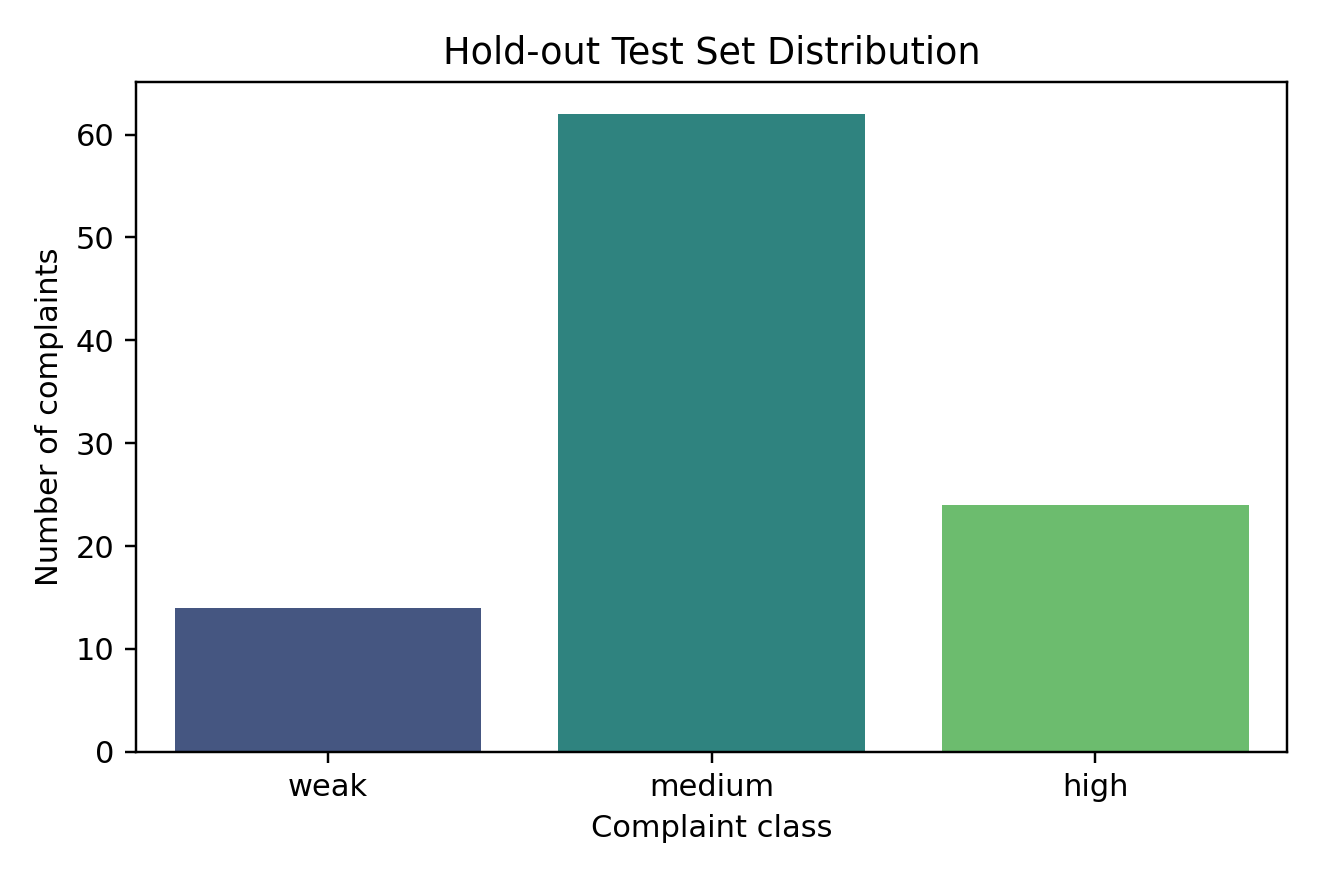
\includegraphics[width=0.72\textwidth]{figures/test_set_distribution.png}
  \caption{Distribution of complaint classes in the 20\% stratified hold-out test set}
  \label{fig:test_distribution}
\end{figure}

\section{Label Definition}
The target label has three classes. Weak complaints represent low-severity or low-validity cases. Medium complaints represent cases that require attention but may not demand immediate action. High complaints represent cases with stronger validity, urgency, or public-risk signals.

The backend documentation defines complaint score as:
\begin{equation}
ComplaintScore = 0.6 \times Validity + 0.4 \times Priority.
\end{equation}
Operational labels are assigned using score thresholds: high for scores greater than or equal to 0.70, medium for scores from 0.40 to 0.69, and weak for scores below 0.40. This relationship matters for interpretation. Since validity and priority help define the operational label, they naturally carry strong predictive information. They are appropriate for a backend decision-support model, but the result should not be read as proof that text alone solves the task.

\section{Complaint Examples}
Table \ref{tab:complaint_examples} presents representative examples showing Bengali, English, and Banglish variation. Personal identifiers are omitted.

\begin{table}[H]
\centering
\caption{Representative complaint examples}
\label{tab:complaint_examples}
\small
\begin{tabular}{p{0.16\textwidth}p{0.58\textwidth}p{0.15\textwidth}}
\toprule
\textbf{Language} & \textbf{Complaint text} & \textbf{Class}\\
\midrule
Bengali & \bn{সয়াবিন তেল এর গুণমান খারাপ ছিল। পচা এবং দুর্গন্ধযুক্ত।} & High\\
English & The product quality was very poor. Rotten and smelly. & High\\
Banglish & Dokane expired dim bikri kore. Swasther jonno khotikar. & High\\
Mixed & Bashi morich bikri koreche. Taka ferot chay nai. & Medium\\
\bottomrule
\end{tabular}
\end{table}

\section{Ethical Considerations}
Complaint data can contain personal information, shop names, and allegations. A complaint classification system must be designed with privacy and fairness in mind. This study uses exported research data for model evaluation and does not require disclosure of personally identifiable information in the thesis text. Examples are limited and should be anonymized in any public version.

The classifier should not be used as the sole authority for legal or punitive decisions. It should support prioritization and routing, while human administrators retain responsibility for final decisions. This is particularly important when model predictions are wrong or when a complaint contains unusual details not captured by the training data.

\section{Data Privacy Discussion}
Data privacy requires three practical steps: minimize unnecessary personal data, restrict access to raw complaints, and log model outputs responsibly. If deployed, the system should store predictions with timestamps and model version identifiers so that decisions can be audited. Sensitive fields such as customer identifiers and contact details should not be used in the ML feature set unless there is a clear legal and ethical basis. This study uses complaint text, product subcategory, validity, and priority only.

\chapter{Methodology}

\section{Overall Machine Learning Pipeline}
The methodology follows a structured pipeline: data loading, preprocessing, feature extraction, feature fusion, model training, cross-validation, hyperparameter tuning, final hold-out evaluation, and result reporting. Figure \ref{fig:ml_pipeline} gives the full flow.

\begin{figure}[H]
\centering
\begin{tikzpicture}[
  scale=0.82,
  transform shape,
  node distance=0.75cm,
  box/.style={rectangle,draw=black,rounded corners,align=center,minimum width=3.15cm,minimum height=0.75cm,fill=gray!7},
  arr/.style={-{Latex[length=2.4mm]},thick}
]
\node[box] (raw) {Raw complaint records};
\node[box,below=of raw] (norm) {Unicode, punctuation, repeated-character,\\and Banglish normalization};
\node[box,below left=0.7cm and 1.5cm of norm] (text) {Word and character\\TF-IDF};
\node[box,below=0.7cm of norm] (cat) {One-Hot Encoding\\subcategory};
\node[box,below right=0.7cm and 1.5cm of norm] (num) {Standard scaling\\validity, priority};
\node[box,below=2.2cm of norm] (fusion) {ColumnTransformer\\feature fusion};
\node[box,below=of fusion] (model) {Classifiers and\\imbalance handling};
\node[box,below=of model] (eval) {Cross-validation, tuning,\\hold-out evaluation};
\draw[arr] (raw) -- (norm);
\draw[arr] (norm) -- (text);
\draw[arr] (norm) -- (cat);
\draw[arr] (norm) -- (num);
\draw[arr] (text) -- (fusion);
\draw[arr] (cat) -- (fusion);
\draw[arr] (num) -- (fusion);
\draw[arr] (fusion) -- (model);
\draw[arr] (model) -- (eval);
\end{tikzpicture}
\caption{Machine learning pipeline used in the thesis}
\label{fig:ml_pipeline}
\end{figure}

\section{Text Preprocessing Pipeline}
We designed the preprocessing pipeline for Bengali, English, and Banglish complaint text. The steps are:
\begin{enumerate}
  \item Convert missing values to empty strings.
  \item Apply Unicode NFKC normalization.
  \item Lowercase English and Banglish tokens.
  \item Compress repeated characters.
  \item Remove noisy punctuation while preserving Bengali, Latin letters, digits, and spaces.
  \item Replace frequent Banglish marketplace terms using a dictionary.
  \item Optionally remove Bengali stopwords.
\end{enumerate}

The goal is not to over-clean the text. Too much cleaning can remove useful complaint signals. The pipeline removes common noise while preserving domain words such as product names, price terms, expiry terms, and quality terms.

\section{Unicode Normalization}
Unicode normalization converts visually similar character sequences into a consistent representation. We use NFKC normalization. In multilingual text, different input methods can create compatibility characters or inconsistent forms. Normalization reduces unnecessary variation before tokenization and vectorization.

\section{Banglish Normalization}
Banglish normalization maps frequent Romanized marketplace terms to Bengali equivalents. Examples include \textit{dokan} to \bn{দোকান}, \textit{dam} to \bn{দাম}, \textit{taka} to \bn{টাকা}, \textit{chal} to \bn{চাল}, and \textit{nosto} to \bn{নষ্ট}. The dictionary is simple by design, so it can be checked and revised easily. A larger neural transliteration system may be useful later, but this work prioritizes transparency and low-resource deployment.

\section{Stopword Removal}
Stopwords are frequent function words that may carry less class-specific information. We implemented Bengali stopword removal as an optional parameter, and the final Logistic Regression model selected it during hyperparameter tuning. Stopword removal is not always helpful in short texts because even common words can support phrase patterns. For that reason, we treated it as a tunable choice rather than a fixed rule.

\section{TF-IDF Mathematics}
TF-IDF transforms text into numeric vectors by combining local term frequency with corpus-level rarity. We evaluated both word-level and character-level TF-IDF features. Sublinear term frequency is used so that repeated words do not dominate linearly. If $tf$ is the raw term frequency, sublinear scaling uses:
\begin{equation}
tf_{sublinear}=1+\log(tf).
\end{equation}

The final TF-IDF matrix is sparse because each complaint contains only a small subset of possible words or character n-grams. Sparse matrices are memory-efficient and work well with linear classifiers.

\section{Word N-Gram Extraction}
Word n-grams represent sequences of words. A unigram model uses individual words, while a bigram model includes adjacent two-word phrases. For example, ``expired product'' and ``beshi taka'' can be more informative than the words alone. We compared word n-gram ranges $(1,1)$ and $(1,2)$.

\section{Character N-Gram Extraction}
Character n-grams represent subword sequences. The character \texttt{char\_wb} n-gram range $(3,5)$ is used because three-to-five-character fragments can capture meaningful spelling patterns without producing excessively long sequences. Character n-grams are particularly helpful for Banglish spelling variation and incomplete words.

\section{FeatureUnion Explanation}
When word and character TF-IDF are combined, the pipeline uses a \texttt{FeatureUnion}. A FeatureUnion runs multiple feature extractors in parallel and concatenates their outputs. If $X_w$ is the word TF-IDF matrix and $X_c$ is the character TF-IDF matrix, the combined text matrix is:
\begin{equation}
X_{text}=[X_w \; X_c].
\end{equation}
This allows the model to use both complete-token meaning and subword robustness.

\section{Numeric Feature Scaling}
The backend numeric features are validity and priority. These values are scaled using \texttt{StandardScaler} with sparse compatibility. Scaling is useful because models such as Logistic Regression and Linear SVC are sensitive to feature magnitudes. If $\mu$ is the mean and $\sigma$ is the standard deviation, scaling is:
\begin{equation}
z=\frac{x-\mu}{\sigma}.
\end{equation}

\section{One-Hot Encoding}
Product category or subcategory is categorical. One-Hot Encoding converts each category into a binary feature. Unknown categories are ignored during transformation, so the model can process categories that were not seen during training. In our ablation study, product category did not improve this dataset and reduced weighted F1 when added to text.

\section{Cross-Validation Methodology}
Stratified five-fold cross-validation was used to estimate model performance. Stratification preserves class proportions in each fold. For each fold, the model trains on four parts and validates on the remaining part. If the fold metric values are $m_1,m_2,\ldots,m_5$, the mean and standard deviation are:
\begin{equation}
\bar{m}=\frac{1}{5}\sum_{i=1}^{5}m_i,
\end{equation}
\begin{equation}
s=\sqrt{\frac{1}{5}\sum_{i=1}^{5}(m_i-\bar{m})^2}.
\end{equation}

\section{Hyperparameter Tuning}
We used RandomizedSearchCV to tune candidate models. Randomized search samples combinations from a defined parameter space and evaluates them with cross-validation. It is more efficient than exhaustive grid search when several hyperparameters exist. The tuned parameters included TF-IDF maximum features, word n-gram range, optional Bengali stopword removal, Logistic Regression $C$, Linear SVC $C$, and Random Forest tree parameters.

\section{Class Imbalance Handling}
The dataset is imbalanced, and the medium class is the majority class. Logistic Regression and Linear SVC used \texttt{class\_weight='balanced'}, which increases the loss contribution of minority classes. We also tested SMOTE. To avoid leakage, we placed SMOTE inside the training pipeline so that synthetic samples were created only from the training portion of each fold.

\section{Ablation Study Methodology}
An ablation study removes or adds feature groups to measure their contribution. Four feature sets were evaluated:
\begin{enumerate}
  \item Text only.
  \item Text plus product category.
  \item Text plus backend numeric features.
  \item Full hybrid feature set: text, product category, and numeric features.
\end{enumerate}
The ablation study is central to this work because it shows that backend numeric features are the main reason performance improves.

\section{Why Linear Models Outperform Random Forest on Sparse TF-IDF}
Sparse TF-IDF vectors have many dimensions and many zero values. Linear models can assign weights directly to useful terms and learn a separating hyperplane. Random Forest models split features one at a time, so they may struggle when useful evidence is spread across many sparse dimensions. In small datasets, tree ensembles may also overfit local patterns or fail to find stable splits. This helps explain why Linear SVC and Logistic Regression outperformed Random Forest in the experiments.

\section{Pseudocode}
\begin{lstlisting}[caption={Pseudocode for the experimental pipeline},label={lst:pseudocode}]
Input: Complaint dataset D with text, subcategory, validity, priority, label
Output: Evaluation tables, final classifier, confusion matrix

1. Load D from complaints_full.csv
2. Drop rows with missing required fields
3. Map labels: weak -> 0, medium -> 1, high -> 2
4. Create stratified 80/20 train-test split
5. For each TF-IDF variant:
      preprocess text
      extract features
      evaluate Linear SVC with 5-fold StratifiedKFold
6. For each classifier and imbalance setting:
      build hybrid feature pipeline
      optionally apply SMOTE inside training folds
      evaluate with 5-fold StratifiedKFold
7. Tune Logistic Regression, Linear SVC, and Random Forest
8. Select best tuned model family by weighted F1
9. Run ablation study using best tuned settings
10. Fit final model on training split
11. Evaluate final model on hold-out test split
12. Save reports, tables, and visualizations
\end{lstlisting}

\chapter{Implementation}

\section{Development Environment}
We developed the implementation in Python using a CPU-friendly machine learning stack. The main training script is located at \texttt{ML\_Model\_Training/src/pipeline.py}. The dataset is stored at \texttt{ML\_Model\_Training/data/complaints\_full.csv}, and the generated metrics and figures are stored in \texttt{ML\_Model\_Training/results/}.

\section{Python Ecosystem}
We selected Python because it provides strong libraries for data processing, machine learning, evaluation, and visualization. The main libraries are Scikit-learn, Imbalanced-learn, NumPy, Matplotlib, Seaborn, and Pandas. Scikit-learn provides the pipeline, vectorizer, classifier, and cross-validation tools. Imbalanced-learn provides SMOTE and pipeline support for leakage-safe oversampling.

\section{Scikit-Learn}
We used Scikit-learn for \texttt{TfidfVectorizer}, \texttt{ColumnTransformer}, \texttt{FeatureUnion}, \texttt{LogisticRegression}, \texttt{LinearSVC}, \texttt{RandomForestClassifier}, \texttt{VotingClassifier}, \texttt{StratifiedKFold}, \texttt{cross\_validate}, and \texttt{RandomizedSearchCV}. Pipelines are important here because preprocessing, feature extraction, scaling, oversampling, and classification are handled as one reproducible object.

\section{Imbalanced-Learn}
Imbalanced-learn provides the pipeline that can place SMOTE between feature extraction and classification. This is needed because Scikit-learn's standard pipeline does not treat oversampling as a typical transformer. By placing SMOTE inside the cross-validation workflow, the implementation prevents validation data from influencing synthetic training samples.

\section{Supabase Integration}
Supabase PostgreSQL stores the complaint data. We used the exported CSV for offline model training and evaluation. In a deployment setting, a backend service can load the trained model and classify new complaints after the backend computes validity and priority. The Supabase table remains the source of operational data, while the ML model adds decision-support predictions.

\section{Data Loading}
The data-loading function reads the CSV file, checks required columns, removes incomplete rows, maps class labels to integers, and returns the feature and target matrices. The relevant feature columns are complaint description, subcategory name, validity, and priority.

\begin{lstlisting}[language=Python,caption={Data-loading structure from the training pipeline},label={lst:data_loading}]
required_columns = [
    "complaint_description",
    "complaint_classification",
    "subcategory_name",
    "validity",
    "priority",
]
df = df.dropna(subset=required_columns).copy()
df["target"] = df["complaint_classification"].map(CLASS_MAPPING)
X = df[["complaint_description", "subcategory_name", "validity", "priority"]]
y = df["target"]
\end{lstlisting}

\section{Pipeline Implementation}
The feature transformer uses \texttt{ColumnTransformer}. The text column is processed by the normalizer and TF-IDF pipeline. The product subcategory is processed by One-Hot Encoding when included. Validity and priority are scaled when numeric features are included.

\begin{lstlisting}[language=Python,caption={Simplified hybrid feature transformer},label={lst:feature_transformer}]
transformers = [
    ("text", build_text_pipeline(...), "complaint_description")
]

if feature_set in {"text_category", "full"}:
    transformers.append(
        ("category", OneHotEncoder(handle_unknown="ignore"), ["subcategory_name"])
    )

if feature_set in {"text_numeric", "full"}:
    transformers.append(
        ("numeric", StandardScaler(with_mean=False), ["validity", "priority"])
    )
\end{lstlisting}

\section{Model Training Implementation}
Each model is wrapped in the same pipeline interface. This keeps preprocessing and feature representation comparable across classifiers. Logistic Regression and Linear SVC use balanced class weights. Random Forest is tested with class weighting and tree hyperparameters.

\section{Evaluation Implementation}
The evaluation reports accuracy, weighted precision, weighted recall, and weighted F1. Weighted metrics fit this dataset because the classes are imbalanced and each class should contribute according to its support. The final hold-out report also includes class-wise precision, recall, and F1.

\section{Visualization Generation}
The pipeline generates a class distribution plot, confusion matrix, two-dimensional SVD projection of transformed features, and K-Means cluster projection. These figures are used in Chapter 6 to support interpretation. The SVD plots are exploratory visualizations, not primary evidence of classifier performance.

\section{Training Workflow Diagram}
\begin{figure}[H]
\centering
\begin{tikzpicture}[
  node distance=0.85cm,
  box/.style={rectangle,draw=black,rounded corners,align=center,minimum width=3.2cm,minimum height=0.75cm,fill=gray!7},
  arr/.style={-{Latex[length=2.4mm]},thick}
]
\node[box] (split) {Stratified\\train-test split};
\node[box,below=of split] (cv) {Five-fold\\cross-validation};
\node[box,below left=0.8cm and 1.2cm of cv] (compare) {Model and TF-IDF\\comparison};
\node[box,below right=0.8cm and 1.2cm of cv] (tune) {Randomized\\hyperparameter search};
\node[box,below=2.2cm of cv] (final) {Final tuned\\Logistic Regression};
\node[box,below=of final] (report) {Reports, tables,\\and figures};
\draw[arr] (split) -- (cv);
\draw[arr] (cv) -- (compare);
\draw[arr] (cv) -- (tune);
\draw[arr] (compare) -- (final);
\draw[arr] (tune) -- (final);
\draw[arr] (final) -- (report);
\end{tikzpicture}
\caption{Training and evaluation workflow}
\label{fig:training_workflow}
\end{figure}

\section{Deployment Possibilities}
The trained model can be deployed as a backend service in several ways. It can run as a Python microservice called from the Node.js or application backend. It can also be serialized with \texttt{joblib} and loaded into a scheduled batch job that classifies new complaints. Because the selected model is Logistic Regression with TF-IDF and two numeric features, inference is lightweight and CPU-friendly. This makes it suitable for modest cloud instances and government systems where GPU access is limited.

\chapter{Results and Analysis}

\section{Evaluation Metrics}
We use accuracy, weighted precision, weighted recall, and weighted F1. Precision measures how many predicted examples of a class are correct. Recall measures how many actual examples of a class are found. F1 is the harmonic mean of precision and recall:
\begin{equation}
F1=2\times\frac{Precision\times Recall}{Precision+Recall}.
\end{equation}
Weighted F1 averages class F1 scores by class support, making it suitable for imbalanced datasets.

\section{Baseline Random Forest Results}
The original Random Forest baseline achieved 58.00\% accuracy and 0.58 weighted F1 on the same 20\% hold-out test split. The weak class F1 was approximately 0.30. This result showed that the initial model was not sufficient for reliable triage, especially for minority-class behavior.

After improving preprocessing, feature extraction, model comparison, imbalance handling, tuning, and ablation, the best final model achieved much stronger performance. This gain came from model and feature design, not from adding more data.

\section{Improved Logistic Regression Results}
The final selected model was tuned Logistic Regression using normalized text and backend numeric features. It achieved 86.00\% hold-out accuracy and 0.8594 weighted F1. Table \ref{tab:final_report} gives the class-wise performance.

\begin{table}[H]
\centering
\caption{Final hold-out classification report for tuned Logistic Regression}
\label{tab:final_report}
\begin{tabular}{lrrrr}
\toprule
\textbf{Class} & \textbf{Precision} & \textbf{Recall} & \textbf{F1-score} & \textbf{Support}\\
\midrule
Weak & 0.9231 & 0.8571 & 0.8889 & 14\\
Medium & 0.8750 & 0.9032 & 0.8889 & 62\\
High & 0.7826 & 0.7500 & 0.7660 & 24\\
\midrule
Macro average & 0.8602 & 0.8368 & 0.8479 & 100\\
Weighted average & 0.8596 & 0.8600 & 0.8594 & 100\\
\bottomrule
\end{tabular}
\end{table}

The weak and medium classes achieved strong F1 scores, while the high class remained more difficult. The high class had 24 examples in the test split, and six high complaints were misclassified as medium. This suggests that the boundary between medium and high remains a practical challenge.

\section{TF-IDF Comparison Analysis}
Table \ref{tab:tfidf_comparison} presents the five-fold TF-IDF comparison using Linear SVC.

\begin{table}[H]
\centering
\caption{Five-fold TF-IDF comparison using Linear SVC}
\label{tab:tfidf_comparison}
\begin{tabular}{lccc}
\toprule
\textbf{Feature extractor} & \textbf{Accuracy} & \textbf{Weighted F1} & \textbf{F1 std.}\\
\midrule
Character \texttt{char\_wb} (3,5) & 0.8220 & 0.8225 & 0.0286\\
Word unigram + bigram & 0.8220 & 0.8209 & 0.0359\\
Word + character & 0.8100 & 0.8092 & 0.0342\\
Word unigram & 0.8040 & 0.8041 & 0.0432\\
\bottomrule
\end{tabular}
\end{table}

Character n-grams achieved the highest weighted F1 among TF-IDF variants. This supports the idea that subword features help with spelling variation, Banglish text, and mixed-script complaints. Word unigrams and bigrams also performed competitively, which suggests that phrase-level signals such as ``expired product'' or ``beshi taka'' are useful.

\section{Model Comparison Analysis}
Table \ref{tab:model_comparison} reports the classifier and imbalance comparison on the full hybrid feature set.

\begin{table}[H]
\centering
\caption{Five-fold model comparison on the full hybrid feature set}
\label{tab:model_comparison}
\scriptsize
\setlength{\tabcolsep}{3pt}
\begin{tabular}{p{0.23\textwidth}p{0.25\textwidth}ccc}
\toprule
\textbf{Classifier} & \textbf{Imbalance handling} & \textbf{Accuracy} & \textbf{Weighted F1} & \textbf{F1 std.}\\
\midrule
Linear SVC & Class weight & 0.8100 & 0.8092 & 0.0342\\
Voting Ensemble & Class weight & 0.8020 & 0.8013 & 0.0314\\
Logistic Regression & Class weight & 0.7980 & 0.8000 & 0.0291\\
Linear SVC & Class weight + SMOTE & 0.7820 & 0.7814 & 0.0378\\
Voting Ensemble & Class weight + SMOTE & 0.7580 & 0.7601 & 0.0320\\
Logistic Regression & Class weight + SMOTE & 0.7400 & 0.7461 & 0.0344\\
Random Forest & Class weight & 0.6460 & 0.6224 & 0.0492\\
Random Forest & Class weight + SMOTE & 0.6160 & 0.6083 & 0.0309\\
\bottomrule
\end{tabular}
\end{table}

Linear SVC achieved the best default cross-validation score. After tuning, Logistic Regression was selected because it produced the strongest tuned family and the best final hold-out behavior with the selected feature set. Random Forest performed poorly compared with linear models, which matches the sparse TF-IDF explanation in Chapter 4.

\section{Cross-Validation Analysis}
Cross-validation gives a more reliable estimate than a single split because every record is used for validation once. The best default row, Linear SVC without SMOTE, achieved 0.8092 weighted F1 with a standard deviation of 0.0342. The tuned Logistic Regression family achieved 0.8093 weighted F1 during tuning and 0.8249 full-hybrid cross-validation weighted F1 when evaluated using the tuned configuration.

The difference between cross-validation and hold-out performance needs careful reading. The hold-out test set has only 100 examples, so the exact value can vary depending on the split. The stronger conclusion is the repeated pattern: linear models perform better than Random Forest, and numeric backend features greatly improve performance.

\section{SMOTE Analysis}
SMOTE did not improve the results. In every classifier family, SMOTE reduced weighted F1 compared with class weighting alone. A likely reason is that synthetic interpolation in sparse high-dimensional feature space creates artificial vectors that do not match realistic complaint patterns. For small text datasets, class weighting is often safer than oversampling. We still tested SMOTE correctly by applying it only within training folds.

\section{Ablation Study Analysis}
The ablation study is the key result for understanding the system. Table \ref{tab:ablation} shows that text alone achieved only 0.5559 weighted F1. Adding product category reduced performance slightly to 0.5410. Adding numeric backend features increased weighted F1 to 0.8503. The full feature set achieved 0.8249, which is lower than text plus numeric features.

\begin{table}[H]
\centering
\caption{Ablation study with tuned Logistic Regression}
\label{tab:ablation}
\begin{tabular}{lccc}
\toprule
\textbf{Feature set} & \textbf{Accuracy} & \textbf{Weighted F1} & \textbf{F1 std.}\\
\midrule
Text + numeric features & 0.8500 & 0.8503 & 0.0299\\
Full hybrid feature set & 0.8260 & 0.8249 & 0.0247\\
Text only & 0.5580 & 0.5559 & 0.0419\\
Text + product category & 0.5400 & 0.5410 & 0.0328\\
\bottomrule
\end{tabular}
\end{table}

This result shows that complaint text alone did not achieve high performance. The text contains useful signals, but many complaints are short, repetitive, and semantically overlapping. For example, both medium and high complaints may mention poor quality or expired products. Backend validity and priority scores provide structured information that separates severity levels more effectively.

\section{Why Backend Numeric Features Improved Results}
Validity and priority improved results because they represent domain knowledge already computed by the backend. Validity captures whether the complaint appears legitimate according to price or complaint rules. Priority captures urgency, health risk, fraud terms, or quality concern. These scores reduce ambiguity in text. A short complaint saying ``bad product'' may be difficult to classify from text alone, but if the backend priority is high and validity is high, the model can assign a more appropriate severity.

This finding must still be read carefully. Validity and priority contribute to the operational complaint score used to define labels, so they are not independent evidence in the same way raw text is. They are legitimate deployment-time features, but they also mean the model partly learns the backend severity policy. That is acceptable for a decision-support system whose goal is consistent operational triage, but it limits any claim about pure NLP understanding.

\section{Why Product Category Features Reduced Performance}
Product category features reduced performance in the ablation study. Several reasons are possible. First, the dataset has many product subcategories compared with only 500 records, so category features may be sparse and unstable. Second, severity may depend less on the product type and more on validity and urgency. Third, some product categories appear in all severity classes, making category a weak predictor. Finally, category features may introduce noise that competes with stronger numeric features.

\section{Confusion Matrix Analysis}
Figure \ref{fig:confusion_matrix} shows the final confusion matrix. The model correctly classified 12 of 14 weak complaints, 56 of 62 medium complaints, and 18 of 24 high complaints. Most errors occurred between medium and high classes.

\begin{figure}[H]
  \centering
  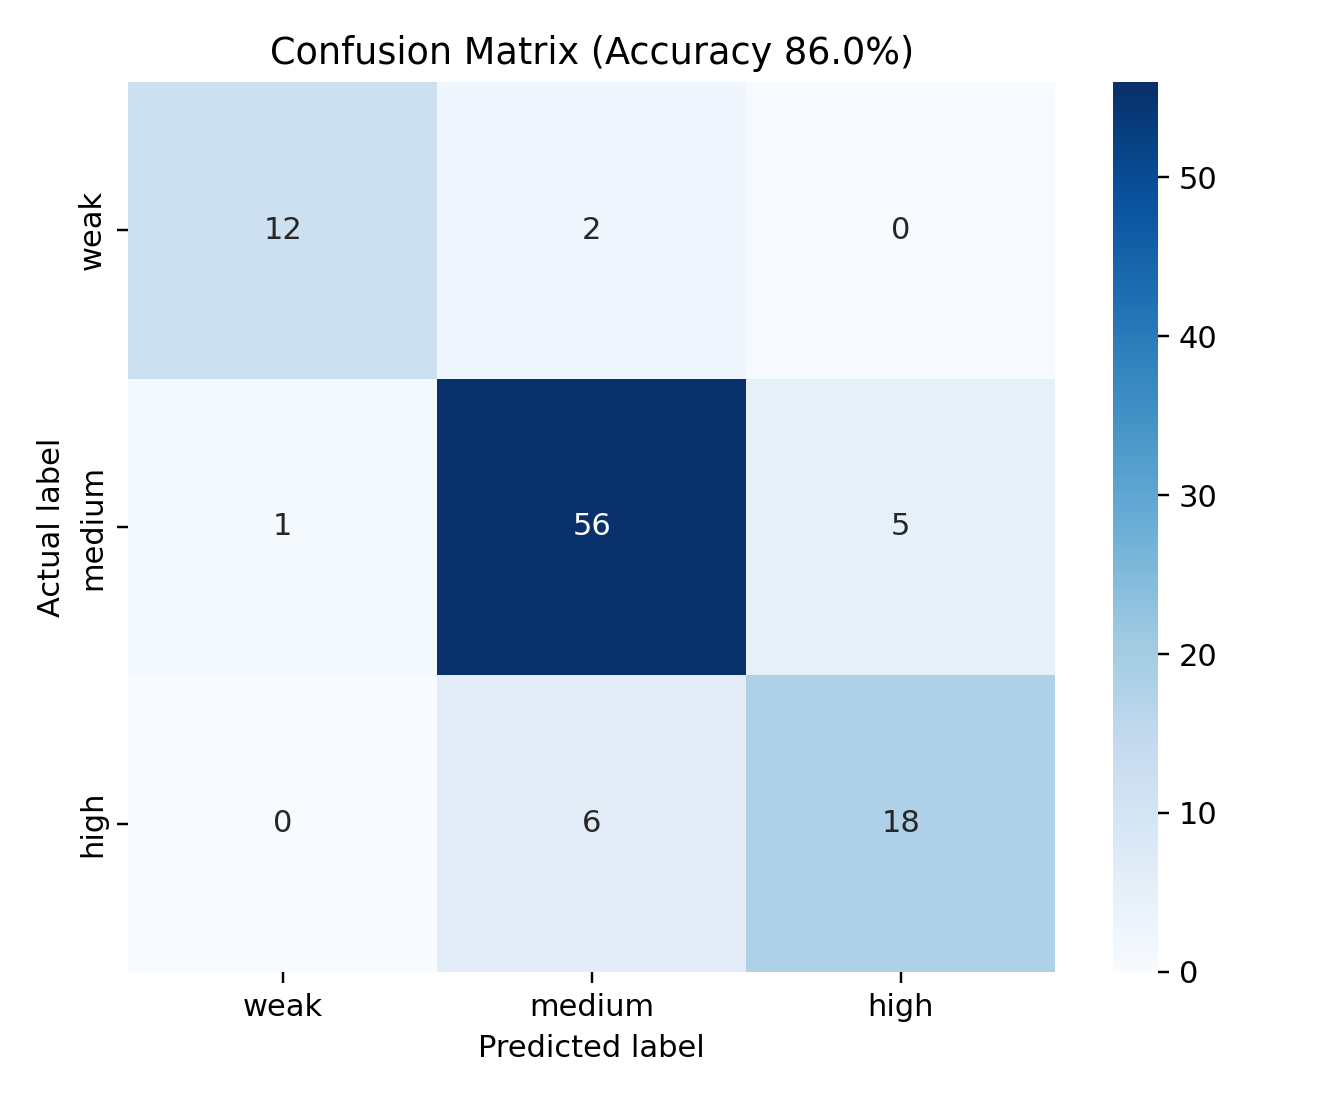
\includegraphics[width=0.68\textwidth]{figures/confusion_matrix.png}
  \caption{Confusion matrix for the final tuned Logistic Regression model}
  \label{fig:confusion_matrix}
\end{figure}

The confusion matrix suggests that the model rarely confuses weak complaints with high complaints. That is useful for triage because the most serious error would be assigning a high-severity complaint to weak. In the hold-out result, no high complaint was predicted as weak. Six high complaints were predicted as medium, so medium-high separation still needs improvement.

\section{Feature Importance Discussion}
For linear models, feature weights can provide interpretability. Positive weights for a class indicate that a feature increases the model's confidence for that class. In this system, backend numeric features are expected to have strong weights because they correlate with severity. Text features related to expiry, health risk, fake products, poor quality, overpricing, and weight manipulation may also contribute.

Unlike Random Forest feature importance, linear model coefficients are more natural for sparse TF-IDF. Future work could export class-wise top weighted terms to help administrators understand model decisions.

\section{Error Analysis}
Errors mainly occur where complaint severity is ambiguous. A complaint may use strong language but have low backend validity. Another complaint may have valid pricing evidence but mild wording. Some Banglish complaints may contain uncommon spellings not covered by the dictionary. Product names in Bengali may also vary in spelling or formatting.

The high class is especially important. A high complaint predicted as medium still receives attention, but perhaps not with the desired urgency. The absence of high-to-weak errors in the test split is a useful sign, but the dataset is small and this should be verified on larger future data.

\section{Class-Wise Analysis}
The weak class improved substantially compared with the original baseline. The final weak F1 score is 0.8889 on the hold-out test set. This improvement is likely because backend validity helps identify low-severity or invalid complaints. The medium class also achieved 0.8889 F1 because it has the largest number of examples and occupies the central score range. The high class achieved 0.7660 F1, which is acceptable but weaker than the other classes.

\section{Statistical Interpretation}
The standard deviations in cross-validation show moderate stability, but the small dataset still affects the estimates. A five-fold standard deviation of about 0.03 in weighted F1 means that fold composition matters. The reported 86.00\% hold-out accuracy should not be treated as a guaranteed production value. It should be read together with cross-validation, ablation, and domain analysis.

\section{SVD and Cluster Visualization}
Figure \ref{fig:svd_projection} shows a two-dimensional SVD projection of the transformed feature space. Figure \ref{fig:kmeans_projection} shows K-Means clusters over the same reduced feature components. These plots help visualize whether classes or clusters show separable structure, but they should not be overinterpreted because high-dimensional data loses information when projected to two dimensions.

\begin{figure}[H]
  \centering
  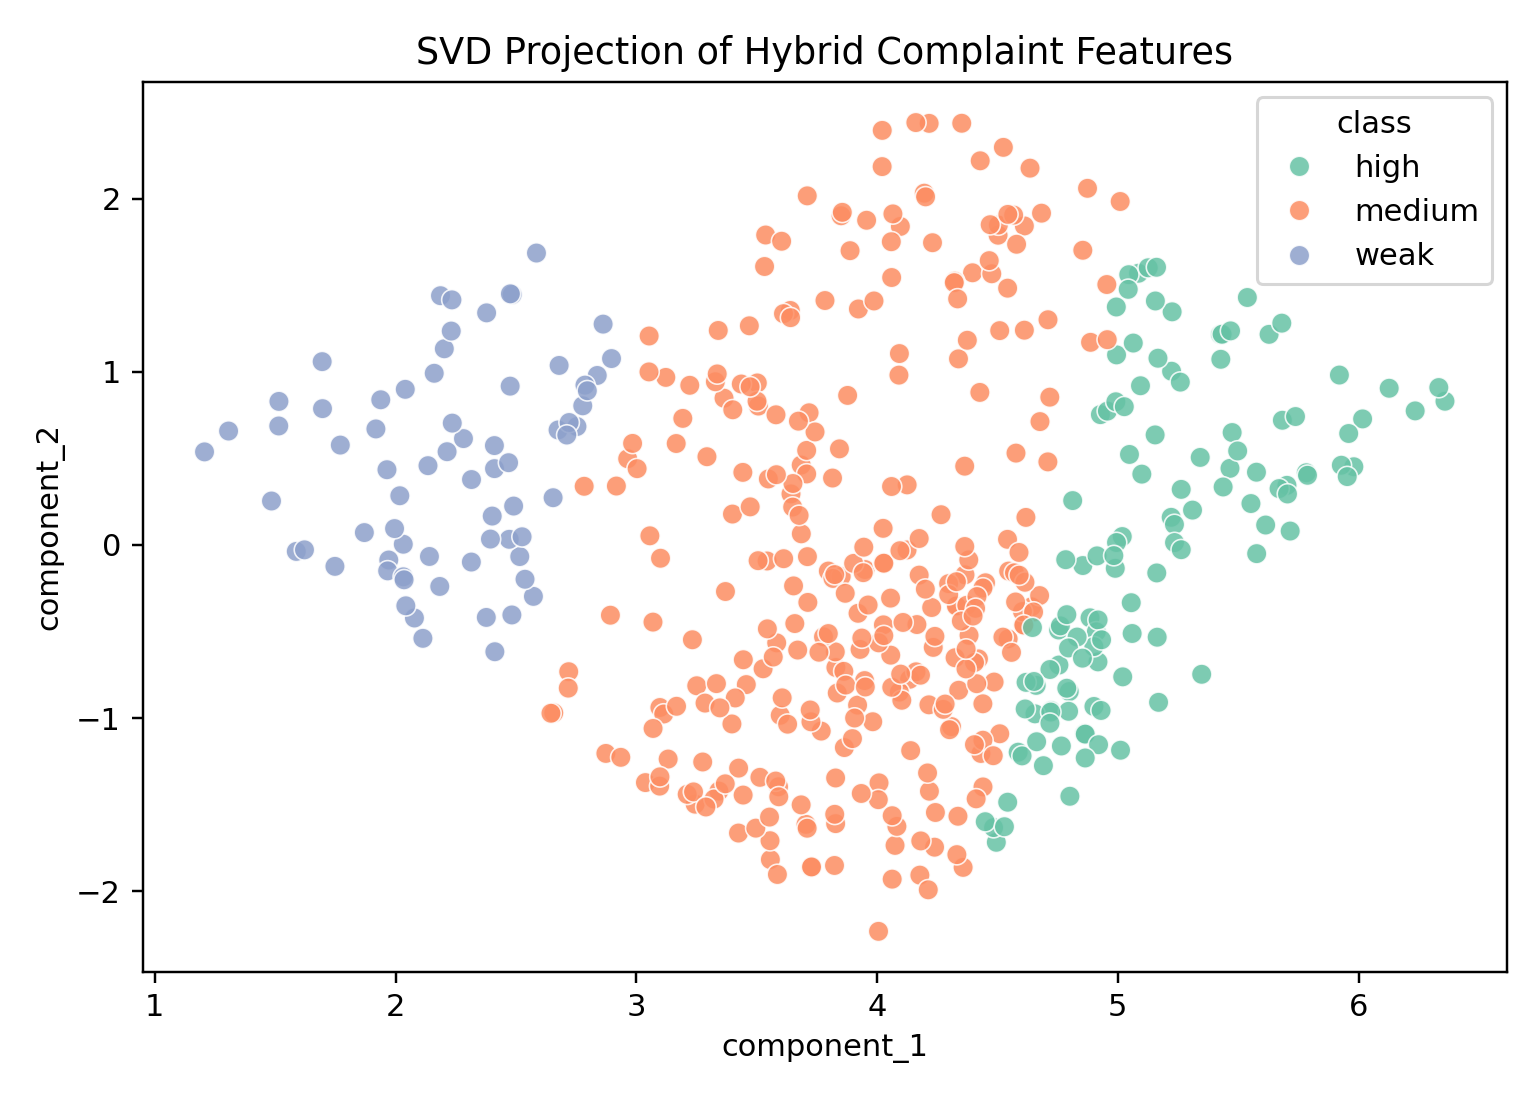
\includegraphics[width=0.72\textwidth]{figures/nlp_pca_clusters.png}
  \caption{Two-dimensional SVD projection of hybrid complaint features}
  \label{fig:svd_projection}
\end{figure}

\begin{figure}[H]
  \centering
  
\includegraphics[width=0.72\textwidth]{figures/kmeans_clusters_pca.png}
  \caption{K-Means cluster projection over transformed hybrid features}
  \label{fig:kmeans_projection}
\end{figure}

\chapter{Discussion}

\section{Interpretation of Results}
The experiment supports one clear reading: a lightweight hybrid model can help classify complaint severity in a Bengali government marketplace context. The strongest evidence comes from the ablation study. Text-only classification was weak, while text plus backend numeric features achieved high weighted F1. For that reason, the system should be described as a hybrid NLP and backend-data classifier, not as a pure NLP solution.

\section{Why the Hybrid System Works}
The hybrid system works because it combines different types of information. Text features capture what the citizen wrote. Character n-grams handle spelling variation and Banglish. Backend numeric features capture operational knowledge that may not be fully expressed in text. A complaint may be short, vague, or emotional, but backend validity and priority can provide structured severity evidence.

\section{Practical Deployment Implications}
During deployment, the model can provide an initial severity prediction after a complaint is submitted and backend scores are computed. Administrators can sort complaint queues by predicted severity, review high-severity cases first, and monitor recurring patterns. The model can also be retrained periodically when new labeled complaints become available.

\section{Lightweight ML Advantages}
The selected approach has several practical advantages. It trains quickly, runs on CPU, requires limited memory, and is easier to inspect than a large transformer. It is also easier to reproduce in a university or government setting. For small datasets, classical models can be more reliable than over-parameterized neural models.

\section{CPU-Friendly Deployment Discussion}
TF-IDF vectorization and Logistic Regression inference are computationally inexpensive. A trained vectorizer and classifier can process many complaints per second on ordinary hardware. This matters for government systems where infrastructure budgets, GPU availability, and maintenance capacity may be limited.

\section{Risks of Backend-Feature Dependency}
The main risk is that backend features may encode the label too directly. In this dataset, validity and priority contribute to complaint score, and complaint score defines severity thresholds. Strong performance therefore partly reflects the model's ability to learn the backend scoring policy. This is not leakage if the same features are available at prediction time, but it limits the claim of independent semantic classification.

To make this risk visible, we report text-only results separately. The text-only result makes clear that language features alone did not produce high performance. Future work should include human-reviewed labels independent of backend score thresholds to test whether the model generalizes beyond the current policy.

\section{Generalization Concerns}
The dataset contains only 500 complaints from one platform context. It may not represent all regions, product types, complaint styles, or administrative policies. Banglish spellings may also vary widely across users. Generalization should be evaluated on future complaints collected after deployment.

\section{Real-World Applicability}
Despite its limits, the system is useful as a triage assistant. It can reduce manual workload by ordering complaints and highlighting likely high-priority cases. It should not replace investigation, enforcement, or final administrative judgment. The best use case is first-level decision support.

\section{Comparison with Transformer-Based Systems}
Transformer models such as BERT and BanglaBERT can capture deeper context and may outperform TF-IDF when enough labeled data and compute are available \cite{devlin2019bert,bhattacharjee2022banglabert}. They are also more expensive to train and deploy. In this work, the lightweight model is a deliberate design choice. It provides strong performance through feature fusion without requiring transformer fine-tuning.

\section{Reviewer Concern: Data Leakage}
Data leakage occurs when information unavailable at prediction time influences training or validation. We avoid common ML leakage by using stratified splits, applying preprocessing inside pipelines, and applying SMOTE only within training folds. Backend-feature dependence is a separate concern. Validity and priority are legitimate prediction-time features, but they are related to label creation. We discuss this openly and treat it as a limitation of independent NLP evaluation.

\section{Reviewer Concern: Backend Features Encoding Labels}
Because complaint labels are generated from complaint score thresholds, and complaint score is calculated from validity and priority, the model can learn a simplified version of the backend scoring rule. This is defensible only if the research objective is operational decision support. It would not be defensible to claim that the model learned complaint severity from language alone. For this reason, the thesis repeatedly distinguishes between text-only performance and hybrid performance.

\section{Reviewer Concern: Small Dataset Size}
A 500-record dataset is small for NLP, especially for three-class classification. We reduce this risk through cross-validation, simple models, regularization, class weighting, and ablation analysis. Larger datasets are still necessary before making strong production claims. This work should be read as a practical undergraduate prototype and a baseline for future expansion.

\chapter{Limitations and Future Work}

\section{Small Dataset Limitations}
The dataset size is the most important limitation. With only 500 records, rare complaint patterns may not be represented. The test split contains only 100 records, so a small number of errors can change the final percentage substantially. Future studies should collect more data over a longer period.

\section{Class Imbalance}
The weak class has fewer examples than the medium class. Although class weighting improved minority-class handling, imbalance remains a concern. Additional weak and high examples should be collected to make the classifier more robust.

\section{Backend-Rule Dependency}
The model depends strongly on backend validity and priority scores. This is useful for operational consistency but limits independent language understanding. If backend rules change, the model may need retraining. If backend scores contain bias or errors, the model may reproduce them.

\section{Banglish Normalization Limitations}
The Banglish dictionary is simple and cannot cover all transliteration variants. Users may write the same Bengali word in many Romanized forms. Future work should evaluate automatic transliteration, phonetic matching, or subword neural models.

\section{Lack of Transformer Benchmarking}
This work intentionally focuses on lightweight classical ML. It does not fine-tune BanglaBERT or multilingual BERT on the dataset. A transformer benchmark would help explain the performance-cost trade-off more completely.

\section{Generalization Limitations}
The dataset comes from a specific marketplace setting. The classifier may not generalize to other government services, legal complaint portals, or private e-commerce platforms without retraining. External validation is needed.

\section{Future Work}
Future work should include:
\begin{enumerate}
  \item Collecting a larger and more diverse complaint dataset.
  \item Creating human-reviewed labels independent of backend score thresholds.
  \item Benchmarking BanglaBERT, multilingual BERT, and other transformer models.
  \item Using active learning so uncertain complaints are prioritized for human labeling.
  \item Investigating online learning for periodic model updates.
  \item Developing a human-in-the-loop dashboard for reviewer feedback.
  \item Adding model explainability reports with top weighted terms and numeric contributions.
  \item Integrating the classifier into the production mobile and backend workflow.
  \item Monitoring fairness, false negatives, and drift after deployment.
\end{enumerate}

\chapter{Conclusion}

\section{Summary of the Work}
This thesis presented a lightweight hybrid NLP and backend-feature based complaint classification system for Bengali government marketplaces. We developed the system using 500 NityMulya complaint records containing Bengali, English, and Banglish text, product subcategory, validity score, priority score, and severity label. The pipeline applied text normalization, Banglish dictionary mapping, TF-IDF feature extraction, feature fusion, class weighting, SMOTE comparison, hyperparameter tuning, cross-validation, ablation, and final hold-out evaluation.

\section{Summary of Findings}
The final tuned Logistic Regression model achieved 86.00\% hold-out accuracy and 0.8594 weighted F1. The ablation study showed that text-only features achieved only 0.5559 weighted F1, while text plus backend numeric features achieved 0.8503 weighted F1. Backend validity and priority features were the major contributors to performance. Product category features did not improve results in this dataset.

\section{Contributions}
The thesis contributes a reproducible, low-resource, deployment-oriented complaint classification pipeline. It shows that classical machine learning can be useful when combined with structured backend features. It also gives a careful analysis of limitations, especially the fact that backend numeric features are related to the operational label definition.

\section{Practical Significance}
For a government marketplace platform, the proposed system can support faster complaint triage, reduce manual workload, and help administrators identify high-priority cases. Because the model is lightweight, it can run on CPU infrastructure and can be integrated into backend services without the cost of transformer deployment.

\section{Final Remarks}
This work shows that practical AI for public-service systems does not always require the largest model. In a low-resource setting, careful preprocessing, feature engineering, backend-data fusion, and honest evaluation can produce a useful decision-support system. The next step is to collect more data, add independent human labels, compare transformer baselines, and evaluate the system in a real administrative workflow.

\appendix

\chapter{Sample Dataset Entries}
\begin{longtable}{p{0.22\textwidth}p{0.43\textwidth}p{0.12\textwidth}p{0.12\textwidth}}
\caption{Sample anonymized complaint records}\\
\toprule
\textbf{Subcategory} & \textbf{Complaint text} & \textbf{Validity} & \textbf{Class}\\
\midrule
\bn{ডিম (ফার্ম)} & Dokane expired \bn{ডিম} bikri kore. Swasther jonno khotikar. & 0.64 & High\\
\bn{এ্যাংকর ডাল} & \bn{এ্যাংকর ডাল} kinte giye protoronar shikar hoyechi. Fake product diyeche. & 0.65 & Medium\\
\bn{আটা (প্যাকেট)} & Dokane expired \bn{আটা} bikri kore. Swasther jonno khotikar. & 0.30 & Medium\\
\bn{সয়াবিন তেল} & \bn{সয়াবিন তেল এর গুণমান খারাপ ছিল। পচা এবং দুর্গন্ধযুক্ত।} & 0.72 & High\\
\bottomrule
\end{longtable}

\chapter{Banglish Normalization Dictionary}
\begin{longtable}{ll}
\caption{Selected Banglish normalization entries}\\
\toprule
\textbf{Banglish token} & \textbf{Normalized form}\\
\midrule
alu & \bn{আলু}\\
bashi & \bn{বাসি}\\
beshi & \bn{বেশি}\\
chal & \bn{চাল}\\
dam & \bn{দাম}\\
dal & \bn{ডাল}\\
dim & \bn{ডিম}\\
dokan & \bn{দোকান}\\
dokandar & \bn{দোকানদার}\\
dudh & \bn{দুধ}\\
expired & \bn{মেয়াদোত্তীর্ণ}\\
fake & \bn{নকল}\\
kharap & \bn{খারাপ}\\
kom & \bn{কম}\\
nosto & \bn{নষ্ট}\\
oil & \bn{তেল}\\
price & \bn{দাম}\\
receipt & \bn{রসিদ}\\
rice & \bn{চাল}\\
taka & \bn{টাকা}\\
\bottomrule
\end{longtable}

\chapter{Hyperparameter Search Space}
\begin{longtable}{p{0.35\textwidth}p{0.5\textwidth}}
\caption{Hyperparameter search space}\\
\toprule
\textbf{Parameter} & \textbf{Candidate values}\\
\midrule
Bengali stopword removal & False, True\\
Word n-gram range & (1,1), (1,2)\\
Word TF-IDF max features & 500, 1000, 2000\\
Character TF-IDF max features & 500, 1000, 2000\\
SMOTE & passthrough, SMOTE(k=3)\\
Logistic Regression $C$ & 0.1, 0.5, 1.0, 2.0, 5.0, 10.0\\
Linear SVC $C$ & 0.1, 0.5, 1.0, 2.0, 5.0, 10.0\\
Random Forest n\_estimators & 100, 200, 300\\
Random Forest max\_depth & None, 8, 12, 20\\
Random Forest min\_samples\_split & 2, 5, 10\\
\bottomrule
\end{longtable}

\chapter{Full Classification Reports}
\begin{table}[H]
\centering
\caption{Confusion matrix rows=true, columns=predicted}
\begin{tabular}{lrrr}
\toprule
 & \textbf{Weak} & \textbf{Medium} & \textbf{High}\\
\midrule
Weak & 12 & 2 & 0\\
Medium & 1 & 56 & 5\\
High & 0 & 6 & 18\\
\bottomrule
\end{tabular}
\end{table}

\begin{table}[H]
\centering
\caption{Hyperparameter tuning results}
\small
\begin{tabular}{lcc}
\toprule
\textbf{Classifier} & \textbf{Best mean weighted F1} & \textbf{Std.}\\
\midrule
Logistic Regression & 0.8093 & 0.0409\\
Linear SVC & 0.8045 & 0.0407\\
Random Forest & 0.6547 & 0.0559\\
\bottomrule
\end{tabular}
\end{table}

\chapter{Source Code Snippets}
\begin{lstlisting}[language=Python,caption={Text normalization logic}]
text = unicodedata.normalize("NFKC", text)
text = text.lower()
text = LATIN_REPEAT_RE.sub(r"\1\1", text)
text = BENGALI_REPEAT_RE.sub(r"\1\1", text)
text = PUNCTUATION_RE.sub(" ", text)

tokens = []
for token in text.split():
    normalized = BANGLISH_MAP.get(token, token)
    if remove_bengali_stopwords and normalized in BENGALI_STOPWORDS:
        continue
    tokens.append(normalized)
\end{lstlisting}

\begin{lstlisting}[language=Python,caption={SMOTE placed inside the training pipeline}]
smote_step = "passthrough"
if use_smote:
    smote_step = SMOTE(k_neighbors=3, random_state=RANDOM_STATE)

pipeline = ImbPipeline(
    steps=[
        ("features", build_feature_transformer(...)),
        ("smote", smote_step),
        ("classifier", build_classifier(model_key)),
    ]
)
\end{lstlisting}

\chapter{Supabase Schema Examples}
\begin{lstlisting}[language=SQL,caption={Simplified complaint table schema}]
CREATE TABLE complaints (
    id UUID PRIMARY KEY DEFAULT gen_random_uuid(),
    created_at TIMESTAMP WITH TIME ZONE DEFAULT CURRENT_TIMESTAMP,
    customer_id UUID NOT NULL,
    shop_id UUID NOT NULL,
    subcategory_id UUID REFERENCES subcategories(id),
    complaint_description TEXT NOT NULL,
    validity DECIMAL(3,2),
    priority DECIMAL(3,2),
    complaint_score DECIMAL(3,2),
    complaint_classification VARCHAR(20)
);
\end{lstlisting}

\backmatter

\begin{thebibliography}{99}
\bibitem{salton1988term}
G. Salton and C. Buckley, ``Term-weighting approaches in automatic text retrieval,'' \textit{Information Processing \& Management}, vol. 24, no. 5, pp. 513--523, 1988.

\bibitem{joachims1998text}
T. Joachims, ``Text categorization with support vector machines: Learning with many relevant features,'' in \textit{Proc. European Conference on Machine Learning}, 1998, pp. 137--142.

\bibitem{cortes1995support}
C. Cortes and V. Vapnik, ``Support-vector networks,'' \textit{Machine Learning}, vol. 20, no. 3, pp. 273--297, 1995.

\bibitem{breiman2001random}
L. Breiman, ``Random forests,'' \textit{Machine Learning}, vol. 45, no. 1, pp. 5--32, 2001.

\bibitem{chawla2002smote}
N. V. Chawla, K. W. Bowyer, L. O. Hall, and W. P. Kegelmeyer, ``SMOTE: Synthetic minority over-sampling technique,'' \textit{Journal of Artificial Intelligence Research}, vol. 16, pp. 321--357, 2002.

\bibitem{pedregosa2011scikit}
F. Pedregosa \textit{et al.}, ``Scikit-learn: Machine learning in Python,'' \textit{Journal of Machine Learning Research}, vol. 12, pp. 2825--2830, 2011.

\bibitem{lemaitre2017imbalanced}
G. Lema{\^i}tre, F. Nogueira, and C. K. Aridas, ``Imbalanced-learn: A Python toolbox to tackle the curse of imbalanced datasets in machine learning,'' \textit{Journal of Machine Learning Research}, vol. 18, no. 17, pp. 1--5, 2017.

\bibitem{devlin2019bert}
J. Devlin, M.-W. Chang, K. Lee, and K. Toutanova, ``BERT: Pre-training of deep bidirectional transformers for language understanding,'' in \textit{Proc. NAACL-HLT}, 2019, pp. 4171--4186.

\bibitem{bhattacharjee2022banglabert}
A. Bhattacharjee, T. Hasan, W. U. Ahmad, K. Samin, M. S. Islam, A. Iqbal, M. S. Rahman, and R. Shahriyar, ``BanglaBERT: Language model pretraining and benchmarks for low-resource language understanding evaluation in Bangla,'' in \textit{Findings of NAACL}, 2022, pp. 1318--1327.

\bibitem{manning2008ir}
C. D. Manning, P. Raghavan, and H. Sch{\"u}tze, \textit{Introduction to Information Retrieval}. Cambridge, U.K.: Cambridge University Press, 2008.

\bibitem{un2022egovernment}
United Nations, \textit{E-Government Survey 2022: The Future of Digital Government}. New York, NY, USA: United Nations, 2022.

\bibitem{postgresql2024docs}
PostgreSQL Global Development Group, \textit{PostgreSQL Documentation}. Accessed: 2026.

\bibitem{supabase2024docs}
Supabase, \textit{Supabase Documentation}. Accessed: 2026.
\end{thebibliography}

\end{document}
